%==============================================================================
% Section 6: Unified Geometric Landau EFT
%==============================================================================
\section{Unified Geometric Landau EFT}
\label{sec:eft}

This section consolidates the results of \S\S\ref{sec:pont}--\ref{sec:spin1}
into a single final effective theory.  The key point is that in the final basis
the quadratic sector is block-diagonally organised and the allowed interaction
terms are described transparently by the invariant basis and representation-
theoretic selection rules.

\subsection{Raw Quadratic Data}

In the raw basis the effective potential is
\begin{equation}
\begin{aligned}
  \Veff &= V_0
    + \tfrac{1}{2}\mu_q^2\,\tr(h^2)
    + \tfrac{1}{2}\mu_\omega^2|\omega|^2
    + \tfrac{1}{2}\mu_\delta^2|\delta|^2
    + m_{\omega\delta}\,\omega\cdot\delta \\
    &\quad + c_\omega\,h_{ij}\omega_i\omega_j
    + c_\delta\,h_{ij}\delta_i\delta_j
    + O(4),
\end{aligned}
\end{equation}
where
\begin{equation}
  \mu_q^2 = 48\pi^2,
  \quad
  \mu_\omega^2 = 52.6379,
  \quad
  \mu_\delta^2 = 3789.9295,
  \quad
  m_{\omega\delta} = -631.6544,
\end{equation}
\begin{equation}
  c_\omega = 105.28,
  \qquad
  c_\delta = 1894.96,
  \qquad
  c_{\omega\delta} = 0 \quad\text{(at the isotropic point)}.
\end{equation}
The raw geometric description is necessary for tracing the geometrical origins but
is redundant as an organiser of physical degrees of freedom.  The final basis is
derived via the physical/auxiliary decomposition of \S\ref{sec:spin1}.

\subsection{Final Quadratic EFT}
\label{sec:eft:quad}

In the final basis the quadratic sector decomposes conceptually as
\begin{equation}
  \mathcal{L}_\mathrm{quad}
  = \mathcal{L}_r
  + \mathcal{L}_{q_A}
  + \mathcal{L}_X
  + \mathcal{L}_Y
  + \mathcal{L}_{\eta,V},
\end{equation}
with
\begin{equation}
  \mathcal{L}_{q_A} = -\frac{1}{2}\mu_q^2 \sum_{A=1}^5 q_A^2,
  \qquad
  \mathcal{L}_X = \frac{1}{2}\dot{X}^T G_\phys \dot{X} - \frac{1}{2} X^T H_\phys X,
  \qquad
  \mathcal{L}_Y = -\frac{1}{2} Y^T H_\mathrm{null} Y.
\end{equation}

Since all 21 mixed Hessian components between $X_k$ and $(q_A,r,\eta)$ vanish,
quadratic decoupling of the spin-1 sector is an exact statement in the final
basis.  All 10 spin-2--torsion cross-Hessian components also vanish at the
isotropic point, and the radial--$V$ cross-Hessian is zero as well.  However,
the radial--$\eta$ cross-Hessian is non-zero ($\approx 118.4$), so the
scalar/torsion subsector forms a coupled $(r,\eta)$ block with $V$ remaining
independent.  Thus the natural block decomposition at quadratic order is
\begin{equation}
  (q_A)\;\oplus\;(X_k)\;\oplus\;(Y_k)\;\oplus\;
  \bigl[(r,\eta)\;\text{block}\;\oplus\;(V)\bigr].
\end{equation}

\begin{figure}[H]
  \centering
  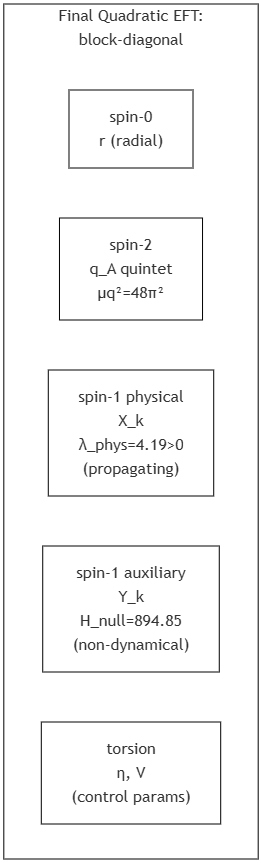
\includegraphics[width=0.4\linewidth]{figures/fig13_final_quadratic_sector.png}
  \caption{Quadratic block organisation of the final sector.  The spin-1 sector
           fully decouples; the spin-2 sector decouples from torsion; the
           scalar/torsion subsector contains a coupled $(r,\eta)$ block.}
  \label{fig:quadratic_block}
\end{figure}

\subsection{Invariant Basis and Selection Rules}

The low-order scalars of the Landau-EFT are organised by the invariant basis
\begin{equation}
  I_2 = \tr(h^2),
  \qquad
  I_3 = h_{ij}\omega_i\omega_j,
  \qquad
  I_4 = \tr(h^3),
  \qquad
  W_2 = \omega_i\omega_i.
\end{equation}
An exact check confirms $I_3 = q_A F_A(\omega)$ in the final $T_A$ basis.  At
quartic order the natural helper invariants are $I_2^2$, $I_2 W_2$, $W_2^2$.

This organisation implies:
\begin{itemize}
  \item Representative allowed cubic terms are $h_{ij}\omega_i\omega_j$ and
        $h_{ij}\delta_i\delta_j$.
  \item Quadratic cross-terms in $X_k$ vanish in the final basis.
  \item Known forbidden terms $H_\mathrm{sym}$ and $K_\mathrm{sym}$ are excluded
        by the representation-theoretic selection rule.
\end{itemize}

\begin{figure}[H]
  \centering
  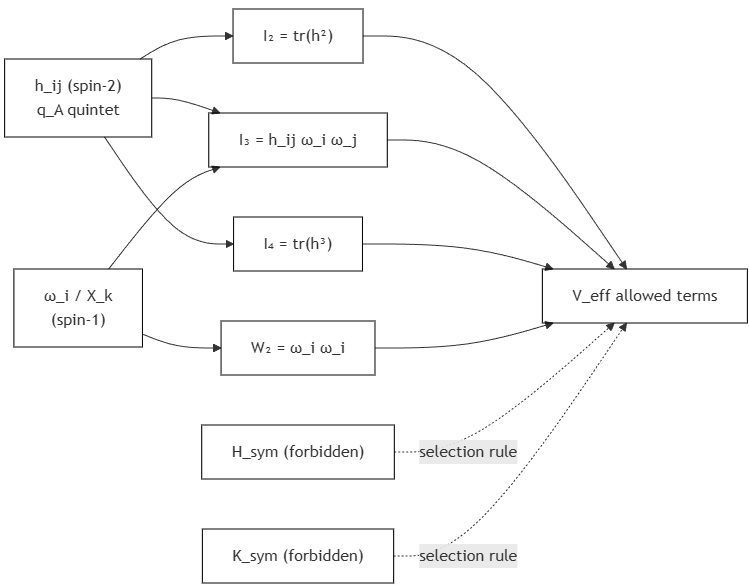
\includegraphics[width=0.75\textwidth]{figures/fig14_EFT_connection_structure.png}
  \caption{Connection structure of low-order invariants in the Landau-EFT.
           Solid arrows indicate allowed terms; dashed arrows indicate terms
           forbidden by selection rules.}
  \label{fig:EFT_conn}
\end{figure}

\subsection{Final Mode Dictionary}
\label{sec:eft:dict}

We recapitulate the mode dictionary adopted in this paper.

\begin{table}[H]
\centering
\begin{tabularx}{\textwidth}{l l l X}
\toprule
Variable & Final classification & Role & Comment \\
\midrule
$r$   & spin-0 & isotropic radius & equilibrium $r_0=3$ \\
$q_A$ & spin-2 & full shear quintet & $\mu_q^2=48\pi^2$ \\
$X_k$ & spin-1 physical  & propagating mixed mode & quadratic decoupled \\
$Y_k$ & spin-1 auxiliary & non-propagating auxiliary & not gauge \\
$\eta$ & spin-0 torsion & AX parameter & input/control \\
$V$   & spin-0 torsion & VT parameter & input/control \\
\bottomrule
\end{tabularx}
\caption{Final mode dictionary.  The raw geometric variables $(\omega_i,\delta_i)$
         are an intermediate description; they are translated to $X_k$ and $Y_k$
         in the final physical dictionary.}
\label{tab:mode_dict}
\end{table}

The block decomposition of the quadratic sector is as given in \S\ref{sec:eft:quad}:
the spin-1 and spin-2 sectors decouple, while the scalar/torsion subsector
retains the coupled $(r,\eta)$ block identified there.

\begin{figure}[H]
  \centering
  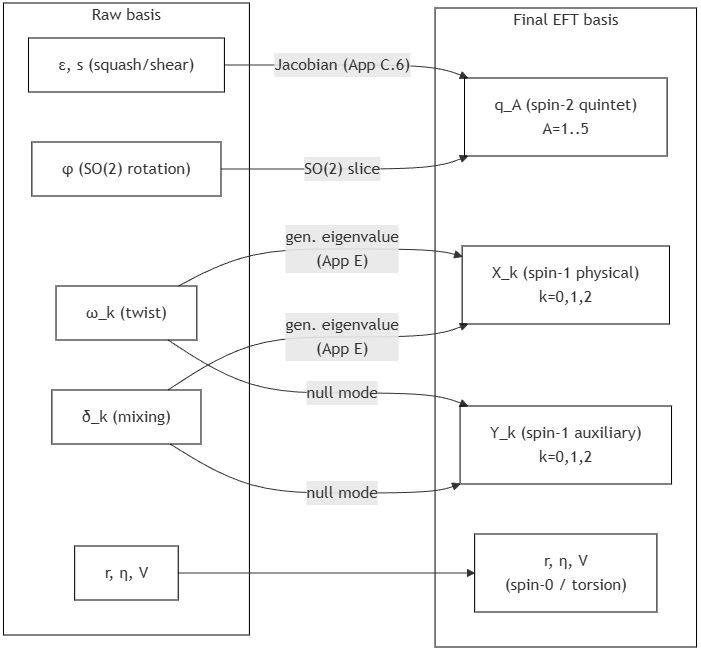
\includegraphics[width=0.85\textwidth]{figures/fig15_assignment_raw2final.png}
  \caption{Overall transformation from raw geometric variables to the final EFT
           basis.  Arrows indicate the assignment of each variable.}
  \label{fig:raw2final}
\end{figure}

\subsection{Interpretation as a Geometric Landau EFT}

From the above results the model can be understood not merely as a description of
a numerical potential in the gravitational minisuperspace, but as a finite-
degree-of-freedom \emph{geometric Landau-EFT}:
\begin{enumerate}
  \item Order-parameter-like geometric degrees of freedom are organised by
        irreducible representations.
  \item The quadratic sector is block-organised into representation-theoretic
        blocks.  The spin-1 sector fully decouples; the scalar/torsion side has
        the refined block structure~--- a coupled $(r,\eta)$ block and an
        independent $V$ direction.
  \item Allowed interactions are described by the invariant basis and
        representation-theoretic selection rules.
\end{enumerate}
This section thus translates the behaviour of the geometric degrees of freedom in
the $\Sthree\times\Sone$ topology of the minisuperspace reduction into a unified
theoretical language.

The cross-Hessian analysis of \S\ref{sec:eft:quad} shows that this block
organisation is exact at quadratic order (see also Appendix~\ref{app:H:numerical}
for the full numerical tables).  In addition, the torsion block $H^{(\eta,V)}$ at
the isotropic point is diagonal and doubly degenerate with positive eigenvalues
($\approx 355.3$), while the coupled $(r,\eta)$ $2\times 2$ block becomes
saddle-point-type (indefinite) in the AX mode, reflecting the flat-direction
nature of $r$, yielding $\lambda_\mathrm{min}<0$.
